\documentclass[a4paper, 12pt]{article}
\usepackage[utf8]{inputenc}
\usepackage[english,russian]{babel}
\usepackage[warn]{mathtext}
\usepackage{graphicx}
\usepackage{float}
\restylefloat{table}
\usepackage{amsmath}
\usepackage{floatflt}
\usepackage[T2A]{fontenc}
\usepackage[left=20mm, top=20mm, right=20mm, bottom=20mm, footskip=10mm]{geometry}

\usepackage{graphicx,calc}
\usepackage{wrapfig}

% Математика
\usepackage{amsmath,amsfonts,amssymb,amsthm,mathtools}

%%% Дополнительная работа с математикой
\usepackage{amsmath,amsfonts,amssymb,amsthm,mathtools} % AMS
\usepackage{icomma} % "Умная" запятая: $0,2$ --- число, $0, 2$ --- перечисление


\tolerance 1414
\hbadness 1414
\emergencystretch 1.5em
\hfuzz 0.3pt        % размер максимального переполнения без warning'a
\widowpenalty=10000 % запрещает одиночную строку абзаца в начале страницы
\vfuzz \hfuzz
\raggedbottom       % если на странице мало содержимого, добавить пустое место в конце, а не в середине страницы



\begin{document}

\begin{titlepage}
	\centering
	\vspace{5cm}
	{\scshape\LARGE московский физико-технический институт (национальный исследовательский университет) \par}
	\vspace{6cm}
	{\scshape\Large Лабораторная работа 3.1.3 \par}
	{\huge\bfseries Измерение магнитного поля земли \par}
	\vspace{1cm}
	\vfill
\begin{flushright}
	{\large Б03-102}\par
	\vspace{0.3cm}
	{\LARGE Куланов Александр}
\end{flushright}
	

	\vfill


	Долгопрудный, 2022 г.
\end{titlepage}

\begin{itemize}
	\item \textbf{Цель работы:} исследовать свойства постоянных неодимовых магнитов: измерить с их
	помощью горизонтальную и вертикальную составляющие индукции магнитного поля Земли и магнитное наклонение.
    \item \textbf{В работе используются:} неодимовые магниты; тонкая нить для изготовления крутильного маятика,
    медная проволока; электронные весы; секундомер; измеритель магнитной индукции; штангенциркуль; брусок,
	линейка и штатив из немагнитных материалов; набор гирь и разновесов.
    
\end{itemize}

\section{Теоретические сведения}

Простейший магнитный диполь может быть образован витком с током или постоянным магнитом. По определению, магнитный момент $\mathfrak{m}$ тонкого витка площадью $S$ с током $I$ равен 
\begin{equation}
	\mathfrak{m} = I\textbf{S}
\end{equation}
где $\textbf{S} = S\textbf{n}$ - вектор площади контура, образующий с направлением тока правовинтовую систему, $\textbf{n}$ - единичный вектор нормали к площадке. Если размеры контура с током или магнитной стрелки малы по сравнению с расстоянием до диполя, то соответствующий магнитный диполь $\mathfrak{m}$ называют \textit{элементарным}, или \textit{точечным}.
Магнитное поле точечного диполя определяется по формуле, анологичной формуле для поля элементарного электрического диполя:
\begin{equation}
    \textbf{B}_\text{дип} = \frac{\mu_0}{4\pi}\left(\frac{3(\mathfrak{m} \cdot \textbf{r})\textbf{r}}{r^5} - \frac{\textbf{m}}{r^3}\right)
    \label{2}
\end{equation}
Во внешнем магнитном поле с индукцией $\textbf{B}$ на точеный магнитный диполь $\mathfrak{m}$ действует механический момент сил 
\begin{equation}
	\textbf{M}=[\mathfrak{m}, \textbf{B}]
\end{equation}
При этом потенциальная энергия которой обладает диполь с постоянным $\mathfrak{m}$, равна 
\begin{equation}
	W = -(\mathfrak{m} \cdot \textbf{B})
\end{equation}
В \textit{неоднородном} внешнем поле выражение для энергии постоянного диполя сохраняется. При этом кроме момента сил на диполь действует ещё и сила 
\begin{equation}
	\textbf{F} = -\nabla W = (\mathfrak{m} \cdot \nabla)\textbf{B}
\end{equation}
Где $\nabla = \left(\frac{\partial}{\partial x},\frac{\partial}{\partial y}, \frac{\partial}{\partial z}\right)$ -- векторный оператор <<набла>> (оператор Гамильтона). В частности, проекция на ось $x$ имеет вид
\begin{equation}
    F_x = \mathfrak{m}_x\frac{\partial B_x}{\partial x} + \mathfrak{m}_y\frac{\partial B_y}{\partial y} + \mathfrak{m}_z\frac{\partial B_z}{\partial z}.
\end{equation}
Таким образом из вышесказанного следует, что \textit{свободный} магнитный диполь в неоднородном магнитном поле ориентируется вдоль силовых линий магнитного поля и втягивается в область более сильного поля, поскольку это ведёт к уменьшению энергии диполя.
Выражения выше, позволяют рассчитать силу взаимодействия магнитов с моментами $\mathfrak{m}_1$ и $\mathfrak{m}_2$. Kогда моменты двух небольших магнитов направлены вдоль соединяющей их прямой: $\mathfrak{m}_{1,2} \| \textbf{r}$, где $\textbf{r}$ - радиус-вектор между ними, они взаимодействуют с силой 
\begin{equation}
    \label{6}
    F_{12}= \mathfrak{m}_1 \frac{\partial{B_2}}{\partial{r}} = \mathfrak{m}_1\frac{\partial{(2\mathfrak{m}_2/r^3)}}{\partial{r}} = -\frac{6 \mathfrak{m}_1\mathfrak{m}_2}{r^4} \;(\text{ед}.\; \text{СГС}).
\end{equation}
(при использовании системы СИ нужно домножить на $\mu_0 / 4\pi$). Здесь магниты притягиваются, если их магнитные моменты сонаправлены, и отталкиваются, если направлены противоположно.
Если магнитные моменты направлены перпендикулярно соединяющей их прямой: $\mathfrak{m}_{1,2} \perp \textbf{r}$, то нетрудно показать, что сила их взаимодействия окажется в два раза меньшей и будет иметь противоположный знак: 
\begin{equation}
	F_{12} = \frac{3\mathfrak{m}_1 \mathfrak{m}_2}{r^4}\;(\text{ед}.\; \text{СГС})
\end{equation}

\section{Экспериментальная установка}
\subsection{Неодимовые магниты}
В работе используются неодимовые магниты шарообразной формы. Важно, чтобы вещество из которого они изготовлены, было \textit{магнитожёстким} материалом и чтобы шары были намагничены однородно.


<<Магнитожесткость>> материала означает, что магнитные моменты шаров в процессе работы не изменяются под действием внешних магнитных полей, т. е. шар ведет себя как постоянный (<<жесткий>>) диполь. В том числе, магнитные моменты не изменяются при контакте магнитов друг с другом.

Магнитное поле однородного намагниченного шара радиусом $R$ может быть вычислено точно. На расстояниях $r \geq R$ от центра шара оно совпадает с полем \textit{точечного} магнитного диполя, расположенного в центре, магнитный момент $\mathfrak{m}$ которого совпадает с полным моментом шара. Внутри шара магнитное поле однородно. Hетрудно получить, что при $r < R$
\begin{equation}
	\textbf{B}_{0} = \frac{\mu_0 \mathfrak{m}}{2\pi R^3}
\end{equation}
В качестве ещё одной характеристики материала магнита используют остаточную \textit{намагниченность} $\textbf{M}$. По определению, намагниченность равна \textit{объёмной плотности магнитного момента, поэтому для однородного намагниченного шара}
\begin{equation}
	\mathfrak{m}= \textbf{M}V
\end{equation}
где $\displaystyle V = \frac{4\pi}{3}R^3$ - объём магнита. Величину $\textbf{B}_r = \mu_0 \textbf{M}$ называют остаточной индукцией материала.
Из сказанного выше нетрудно видеть, что индукция $\textbf{B}_p$ \textit{на полсюсах} однородно намагниченного шара направлена по нормали к поверхности и совпадает поэтому с индукцией внутри шара $\textbf{B}_p = \textbf{B}_0$. Величина $B_p$ связана с остаточной индукцией $B_r$ соотношением
\begin{equation}
	B_p = B_o = \frac{2}{3}B_r
\end{equation}

\subsection{Определение магнитного момента магнитных шариков}

\textbf{Метод А.} Величину магнитного момента $\mathfrak{m}$ двух одинаковых шариков можно рассчитать, зная их массу $m$ и определив максимальное расстояние $r_{max}$, на котором они еще удерживают друг друга в поле тяжести. При максимальном расстоянии сила тяжести шариков $mg$ равна силе их магнитного притяжения.
\begin{figure}[h]
    \centering
    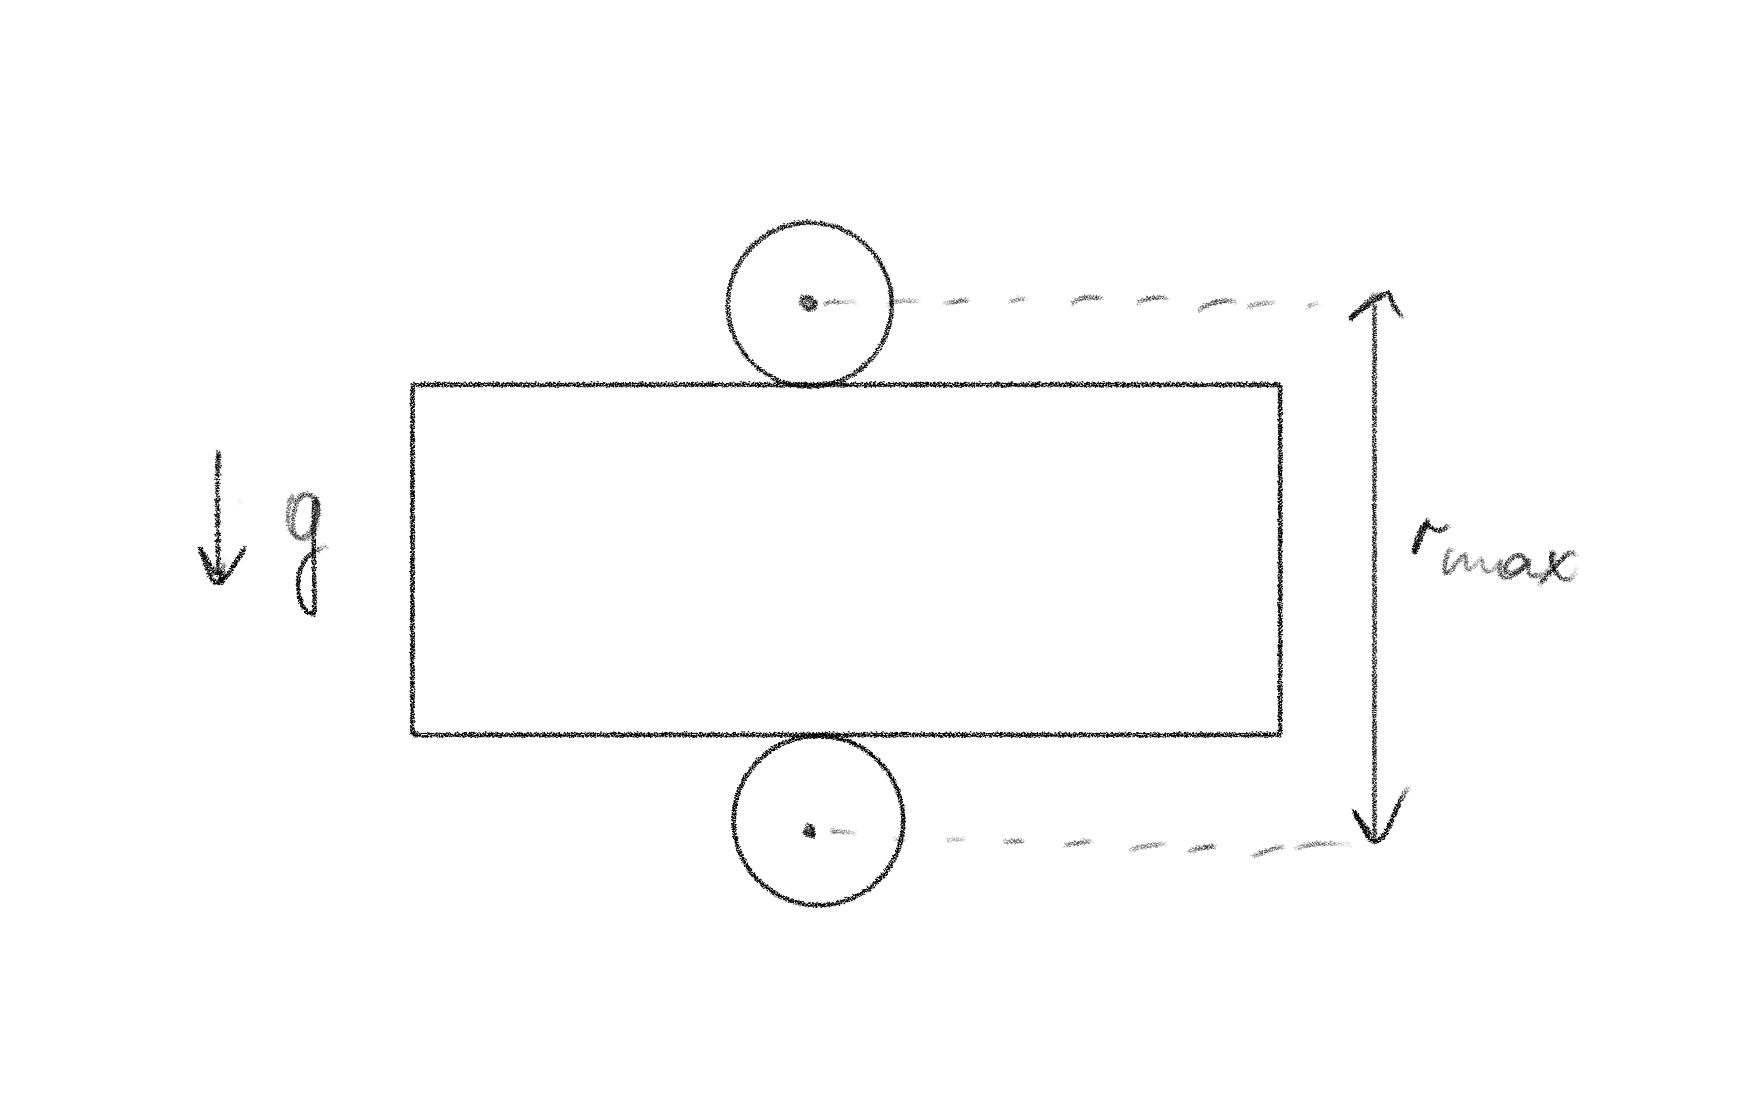
\includegraphics[width=0.7\textwidth]{path1}
    \caption{Метод А}
    \label{fig:path1}
\end{figure}
Когда векторы двух магнитных моментов ориентированы вертикально, из (\ref{6}) имеем
\begin{equation}
    \mathfrak{m} = \sqrt{\frac{2\pi mgr^4_{max}}{3 \mu_0}} \ \text{(ед. СИ).}
\end{equation}
По величине $\mathfrak{m}$ с помощью (\ref{2}) можно рассичать величину индукции $\textbf{B}$ вблизи любой точки на поверхности шара радиуса $R$. Максимальная величина индукции наблюдается на полюсах.

\textbf{Метод Б.} Величину магнитного момента шариков можно определить также по силе их сцепления. Она определяется как сила, необходимая для разрыва двух сцепившихся магнитных шариков. Сила сцепления максимальна, если шары соединяются своими противоположными полюсами (магнитные моменты сонаправлены).

\begin{wrapfigure}{r}{0.3\textwidth}
	\begin{center}
		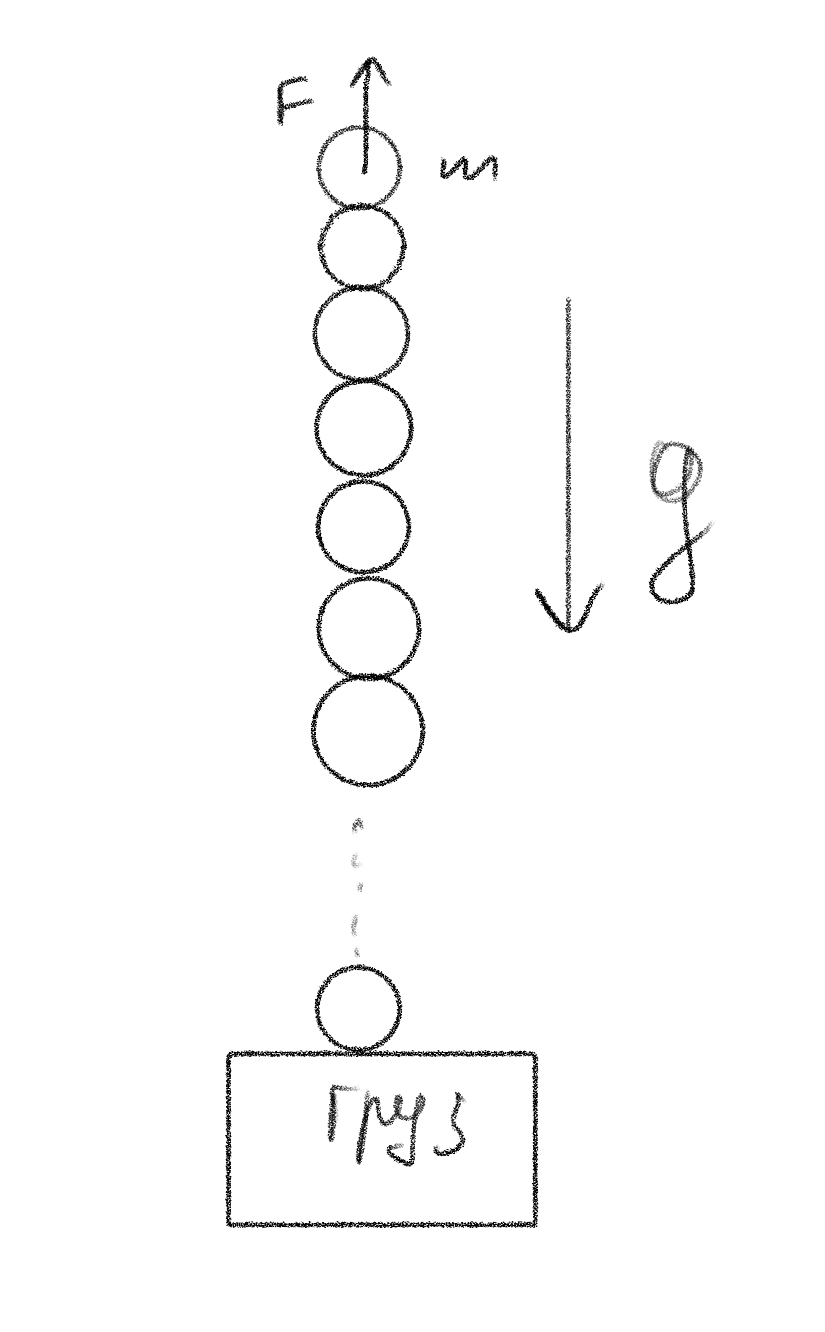
\includegraphics[width=0.3\textwidth]{path2}
		\caption{Метод Б}
	\end{center}
\end{wrapfigure}

Максимальную силу сцепления можно определить по весу магнитной цепочки, 
которую способен удежрать самый верхний магнитный шарик. Если цепь состоит из одинаковых магнитных шариков, 
то при определенённой длине она отрывается от верхнего шарика. При этом учитвая, что сила притяжения убывает как 
$F \propto 1/r^4$, где $r$ - расстояния между центрами шаров, для расчёта прочности цепочки достаточно учитывать 
силу взаимодействия с 3-4 соседями.
Сила сцепления двух одинаковых шаров радиусами $R$ с магнитными момантами $\mathfrak{m}$ равна 
\begin{equation}
        F_0 = \frac{3 \mu_0 \mathfrak{m}^2}{32 \pi R^4}\  \text{(ед. СИ).}    
\end{equation}
Тогда минимальный вес цепочки, при котором она оторвётся от верхнего шарика, равен
\begin{equation}
    F = F_0\left(1 + \frac{1}{2^4} + \frac{1}{3^4} + ... \right) \approx 1,08F_0.
\end{equation}
Отметим, что не обязательно составлять цепочку только из одинаковых шариков: на расстояниях, превышающих 20–30 
диаметров шариков, можно подцепить любой груз. На результат это не повлияет.


\section{Обработка результатов}

Определим величину магнитного момента шарика по методу А. Радиус шарика $r = 0.4 \pm 0.001 \text{ см}$, расстояние между центрами при
отрыве тогда $r_{max} = 2.33\pm 0.001\text{ см}$, масса шарика $m = 0.834 \text{ см}$, тогда
\begin{equation}
    \mathfrak{m} = \sqrt{\frac{2\pi mgr^4_{max}}{3 \mu_0}} = \sqrt{\frac{mgr^4_{max}}{6}} \text{ (ед. СГС)} = 74.7 \pm 2 \text{ эрг/Гс}
\end{equation}
Определим теперь величину момента по методу B. Масса системы без верхнего шарика $m = 317,59 \text{ г}$. Вес системы без верхнего шарика $F = mg = 311236.3 \text{ дин}$.
Тогда имеем
\begin{equation}
	\mathfrak{m} = \sqrt{\frac{8 F_0 r^4}{3}} = \sqrt{\frac{8 F r^4}{3.24}} \text{ (ед. СГС)} = 78.9 \pm 2 \text{ эрг/Гс}
\end{equation}
Найдем индукцию на полюсах шарика:
\begin{equation}
	B_p = B_0 = \frac{2}{3} B_r = \frac{2 \mathfrak{m}}{r^3}
\end{equation}
Для метода А: $B_p = 5534 \pm 110 \text{ Гс}$, для метода B: $B_p = 5844 \pm 117\text{ Гс}$. Значение, полученное магнетометром равно $2140 
\text{ Гс}$. 
Найдем остаточную индукцию: $B_r = 3/2 B_p = 8301 \pm 165 \text{ Гс}$. Табличное значение около $11000 \text{ Гс}$

Определим горизонтальную составляющую магнитного поля Земли. Соберем установку с лямбда-подвесом. Результаты занесем в таблицу \ref{tab:krutilnye}
\begin{table}[h]
	\centering
	\begin{tabular}{|cccccccccc|}
	\hline
	\multicolumn{10}{|c|}{Крутильные колебания}                                                                                                                                                                                                                                                \\ \hline
	\multicolumn{2}{|c|}{5 шаров}                               & \multicolumn{2}{c|}{7 шаров}                                & \multicolumn{2}{c|}{9 шаров}                               & \multicolumn{2}{c|}{11 шаров}                               & \multicolumn{2}{c|}{13 шаров}       \\ \hline
	\multicolumn{1}{|c|}{n}      & \multicolumn{1}{c|}{T,с}       & \multicolumn{1}{c|}{n}      & \multicolumn{1}{c|}{T,c}        & \multicolumn{1}{c|}{n}      & \multicolumn{1}{c|}{T,c}       & \multicolumn{1}{c|}{n}      & \multicolumn{1}{c|}{T,c}        & \multicolumn{1}{c|}{n}      & T,c     \\ \hline
	\multicolumn{1}{|c|}{1}      & \multicolumn{1}{c|}{1,34}    & \multicolumn{1}{c|}{1}      & \multicolumn{1}{c|}{1,52}     & \multicolumn{1}{c|}{1}      & \multicolumn{1}{c|}{1,98}    & \multicolumn{1}{c|}{1}      & \multicolumn{1}{c|}{2,28}     & \multicolumn{1}{c|}{1}      & 4,77  \\ \hline
	\multicolumn{1}{|c|}{2}      & \multicolumn{1}{c|}{1,24}    & \multicolumn{1}{c|}{2}      & \multicolumn{1}{c|}{1,56}     & \multicolumn{1}{c|}{2}      & \multicolumn{1}{c|}{1,76}    & \multicolumn{1}{c|}{2}      & \multicolumn{1}{c|}{2,33}     & \multicolumn{1}{c|}{2}      & 4,58  \\ \hline
	\multicolumn{1}{|c|}{3}      & \multicolumn{1}{c|}{1,1}     & \multicolumn{1}{c|}{3}      & \multicolumn{1}{c|}{1,64}     & \multicolumn{1}{c|}{3}      & \multicolumn{1}{c|}{1,83}    & \multicolumn{1}{c|}{3}      & \multicolumn{1}{c|}{2,32}     & \multicolumn{1}{c|}{3}      & 4,57  \\ \hline
	\multicolumn{1}{|c|}{4}      & \multicolumn{1}{c|}{1,16}    & \multicolumn{1}{c|}{4}      & \multicolumn{1}{c|}{1,65}     & \multicolumn{1}{c|}{4}      & \multicolumn{1}{c|}{1,94}    & \multicolumn{1}{c|}{4}      & \multicolumn{1}{c|}{2,42}     & \multicolumn{1}{c|}{4}      & 4,71  \\ \hline
	\multicolumn{1}{|c|}{5}      & \multicolumn{1}{c|}{1,28}    & \multicolumn{1}{c|}{5}      & \multicolumn{1}{c|}{1,63}     & \multicolumn{1}{c|}{5}      & \multicolumn{1}{c|}{1,86}    & \multicolumn{1}{c|}{5}      & \multicolumn{1}{c|}{2,16}     & \multicolumn{1}{c|}{5}      & 4,93  \\ \hline
	\multicolumn{1}{|c|}{6}      & \multicolumn{1}{c|}{1,2}     & \multicolumn{1}{c|}{6}      & \multicolumn{1}{c|}{1,57}     & \multicolumn{1}{c|}{6}      & \multicolumn{1}{c|}{1,84}    & \multicolumn{1}{c|}{6}      & \multicolumn{1}{c|}{2,47}     & \multicolumn{1}{c|}{6}      & 4,63  \\ \hline
	\multicolumn{1}{|c|}{7}      & \multicolumn{1}{c|}{1,38}    & \multicolumn{1}{c|}{7}      & \multicolumn{1}{c|}{1,67}     & \multicolumn{1}{c|}{7}      & \multicolumn{1}{c|}{2,03}    & \multicolumn{1}{c|}{7}      & \multicolumn{1}{c|}{2,53}     & \multicolumn{1}{c|}{7}      & 4,86  \\ \hline
	\multicolumn{1}{|c|}{8}      & \multicolumn{1}{c|}{1,32}    & \multicolumn{1}{c|}{8}      & \multicolumn{1}{c|}{1,69}     & \multicolumn{1}{c|}{8}      & \multicolumn{1}{c|}{1,85}    & \multicolumn{1}{c|}{8}      & \multicolumn{1}{c|}{1,98}     & \multicolumn{1}{c|}{8}      & 4,57  \\ \hline
	\multicolumn{1}{|c|}{9}      & \multicolumn{1}{c|}{1,25}    & \multicolumn{1}{c|}{9}      & \multicolumn{1}{c|}{1,55}     & \multicolumn{1}{c|}{9}      & \multicolumn{1}{c|}{1,81}    & \multicolumn{1}{c|}{9}      & \multicolumn{1}{c|}{2,45}     & \multicolumn{1}{c|}{9}      & 4,32  \\ \hline
	\multicolumn{1}{|c|}{10}     & \multicolumn{1}{c|}{1,24}    & \multicolumn{1}{c|}{10}     & \multicolumn{1}{c|}{1,6}      & \multicolumn{1}{c|}{10}     & \multicolumn{1}{c|}{2}       & \multicolumn{1}{c|}{10}     & \multicolumn{1}{c|}{2,45}     & \multicolumn{1}{c|}{10}     & 4,89  \\ \hline
	\multicolumn{1}{|c|}{11}     & \multicolumn{1}{c|}{1,25}    & \multicolumn{1}{c|}{11}     & \multicolumn{1}{c|}{1,76}     & \multicolumn{1}{c|}{11}     & \multicolumn{1}{c|}{1,78}    & \multicolumn{1}{c|}{11}     & \multicolumn{1}{c|}{2,12}     & \multicolumn{1}{c|}{11}     &       \\ \hline
	\multicolumn{1}{|c|}{12}     & \multicolumn{1}{c|}{1,17}    & \multicolumn{1}{c|}{12}     & \multicolumn{1}{c|}{1,49}     & \multicolumn{1}{c|}{12}     & \multicolumn{1}{c|}{2,04}    & \multicolumn{1}{c|}{12}     & \multicolumn{1}{c|}{2,2}      & \multicolumn{1}{c|}{12}     &       \\ \hline
	\multicolumn{1}{|c|}{13}     & \multicolumn{1}{c|}{1,19}    & \multicolumn{1}{c|}{13}     & \multicolumn{1}{c|}{1,46}     & \multicolumn{1}{c|}{13}     & \multicolumn{1}{c|}{1,89}    & \multicolumn{1}{c|}{13}     & \multicolumn{1}{c|}{2,5}      & \multicolumn{1}{c|}{13}     &       \\ \hline
	\multicolumn{1}{|c|}{14}     & \multicolumn{1}{c|}{1,26}    & \multicolumn{1}{c|}{14}     & \multicolumn{1}{c|}{1,6}      & \multicolumn{1}{c|}{14}     & \multicolumn{1}{c|}{1,75}    & \multicolumn{1}{c|}{14}     & \multicolumn{1}{c|}{2,5}      & \multicolumn{1}{c|}{14}     &       \\ \hline
	\multicolumn{1}{|c|}{15}     & \multicolumn{1}{c|}{1,27}    & \multicolumn{1}{c|}{15}     & \multicolumn{1}{c|}{1,62}     & \multicolumn{1}{c|}{15}     & \multicolumn{1}{c|}{2,1}     & \multicolumn{1}{c|}{15}     & \multicolumn{1}{c|}{}         & \multicolumn{1}{c|}{15}     &       \\ \hline
	\multicolumn{1}{|c|}{16}     & \multicolumn{1}{c|}{1,33}    & \multicolumn{1}{c|}{16}     & \multicolumn{1}{c|}{1,76}     & \multicolumn{1}{c|}{16}     & \multicolumn{1}{c|}{1,8}     & \multicolumn{1}{c|}{16}     & \multicolumn{1}{c|}{}         & \multicolumn{1}{c|}{16}     &       \\ \hline
	\multicolumn{1}{|c|}{$<T>$} & \multicolumn{1}{c|}{1,24} & \multicolumn{1}{c|}{$<T>$} & \multicolumn{1}{c|}{1,61} & \multicolumn{1}{c|}{$<T>$} & \multicolumn{1}{c|}{1,89} & \multicolumn{1}{c|}{$<T>$} & \multicolumn{1}{c|}{2,33} & \multicolumn{1}{c|}{$<T>$} & 4,68 \\ \hline
	\end{tabular}
	\caption{Крутильные колебания}
	\label{tab:krutilnye}
	\end{table}

Построим график T(n). Учтём, что последний столбец (для 13 шаров) измерен ошибочно, не будем его учитывать при аппроксимации.
\begin{figure}[H]
    \centering
    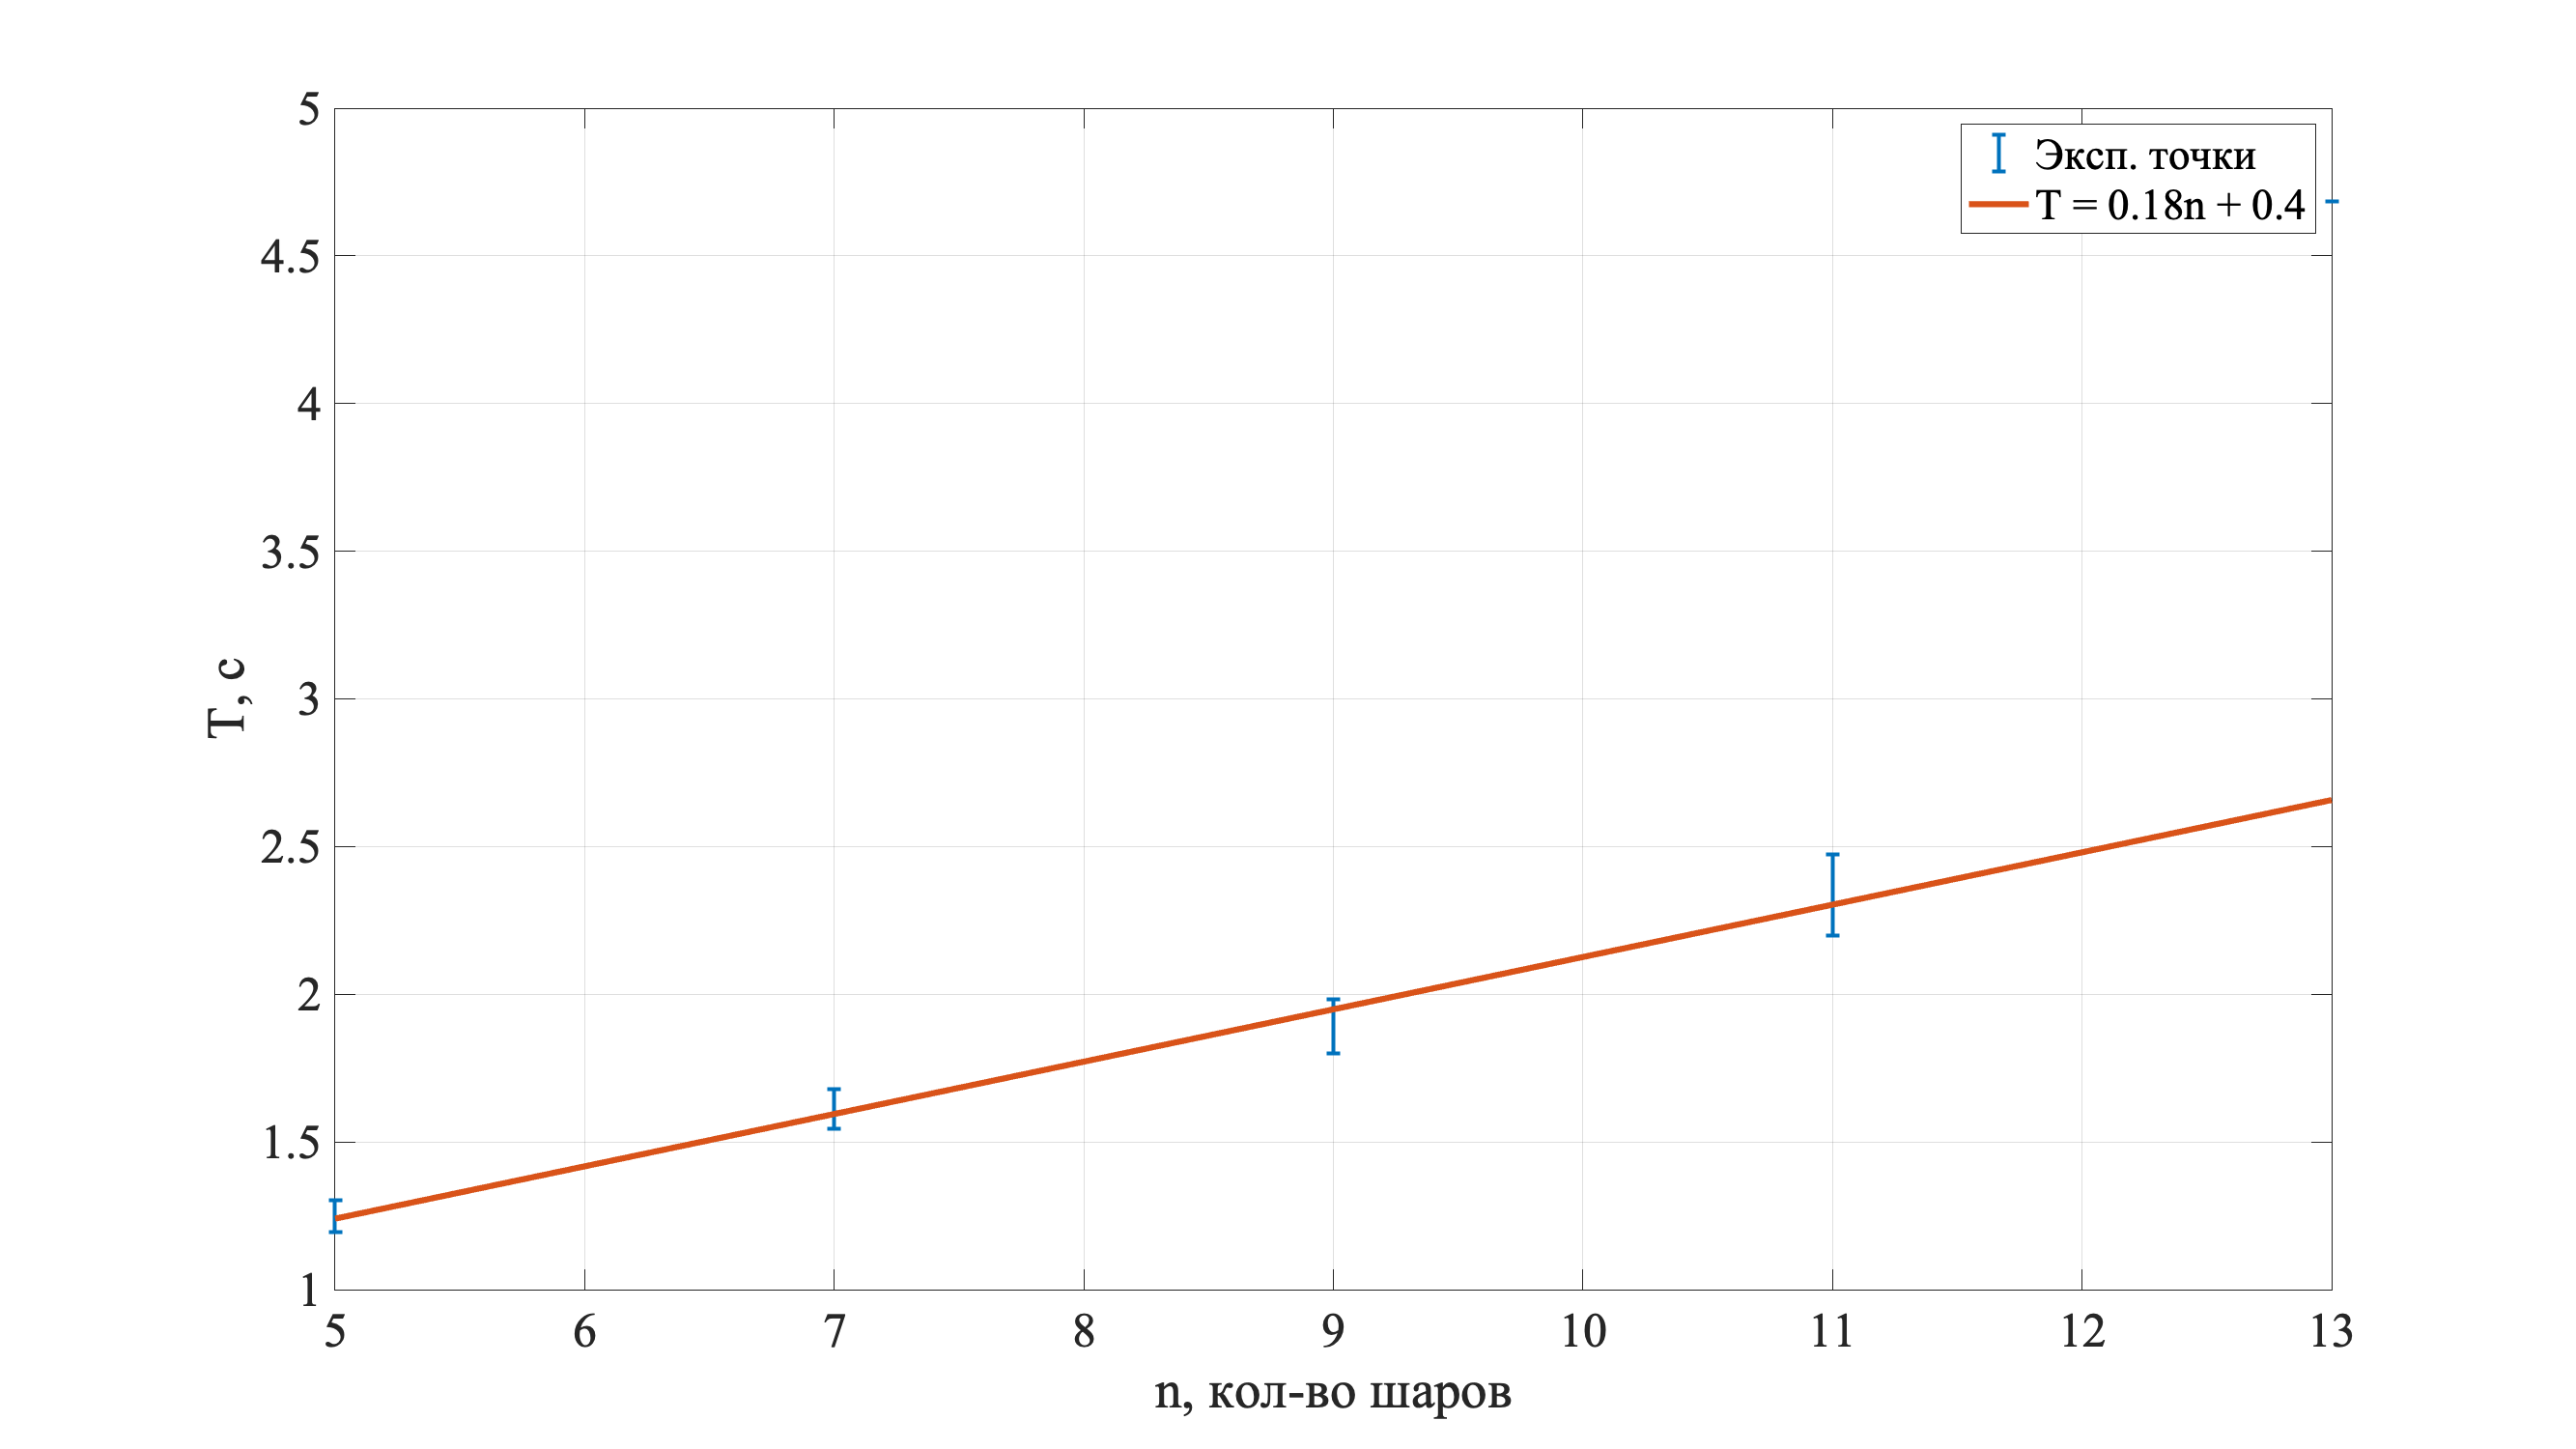
\includegraphics[width=1\textwidth]{plot1}
    \caption{Зависимость T(n)}
    \label{fig:plot1}
\end{figure}
Из графика находим угловой коэфф. k, равный 0.18. Далее можем найти величину горизонтальной составляющей поля Земли:
\begin{equation}
	B_h = \frac{4 \pi^2}{k^2} \frac{mr^2}{3\mathfrak{m}} = 0.41 \pm 0.02 \text{ Гс}
\end{equation}

Определим вертикальную составляющую магнитного поля Земли. Результаты занесем в таблицу \ref{tab:vertic}, где m - масса подвеса, r - плечо:
\begin{table}[H]
	\centering
	\begin{tabular}{|c|c|c|}
	\hline
	m, г  & r, см & M, дин*см \\ \hline
	0,19  & 0,6   & 109.4   \\ \hline
	0,153 & 1,2   & 176.2 \\ \hline
	0,116 & 1,8   & 200.5  \\ \hline
	0,178 & 1,2   & 205.4  \\ \hline
	\end{tabular}
	\caption{Вертикальная составляющая}
	\label{tab:vertic}
\end{table}
Построим график M(n) (рис. \ref{fig:plot2}).
\begin{figure}[h]
    \centering
    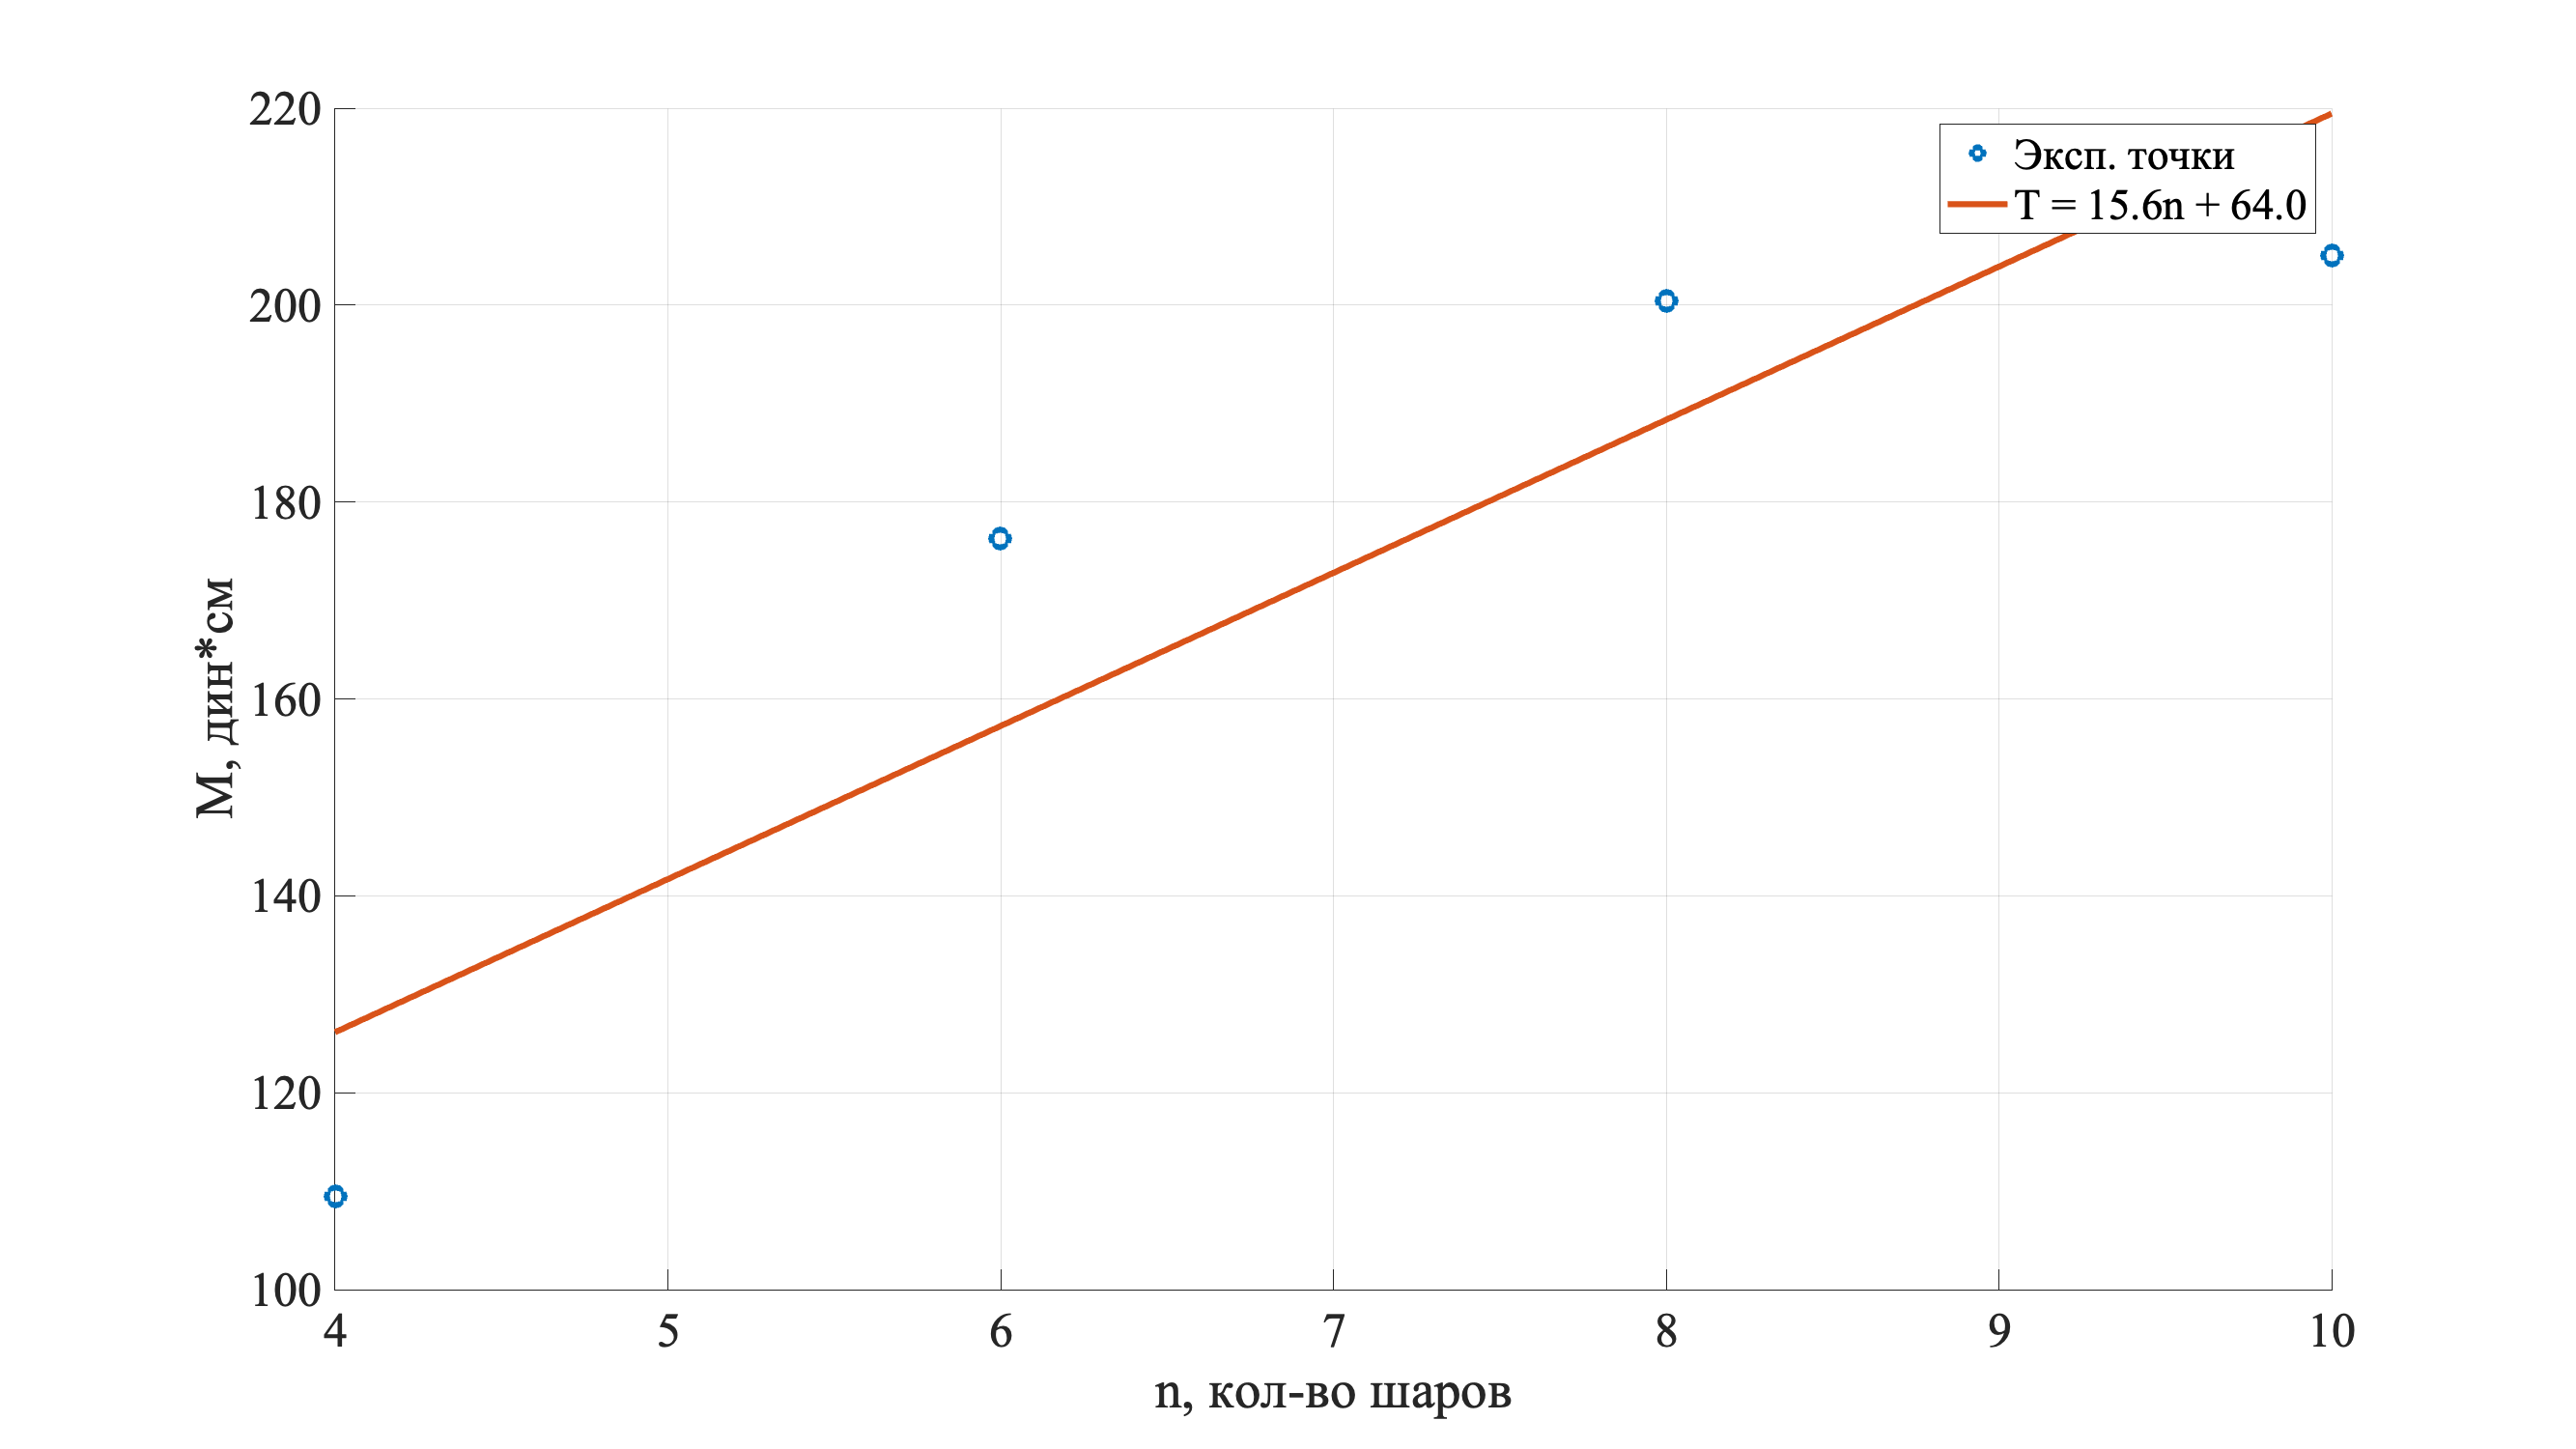
\includegraphics[width=1\textwidth]{plot2}
    \caption{Зависимость M(n)}
    \label{fig:plot2}
\end{figure}
По графику определим угловой коэффициент. Он равен 15.6. Найдем вертикальное поле Земли:
\begin{equation}
	B_{v} = \frac{k}{\mathfrak{m}} = 0.21 \text{ Гс}
\end{equation}
Тогда полное поле равно корню из суммы квадратов:

\begin{equation}
	B = \sqrt{B_v^2 + B_h^2} = 0.46 \pm 0.02 \text{ Гс}
\end{equation}
Наклонение
\begin{equation}
	\beta = arctan(B_h/B_v) = 63 \text{ град.}
\end{equation}
Табличное значение поля для широты Москвы равно $\approx 0.5 \text{ Гс}$


\section{Вывод}
Глядя на результаты работы, можно сказать, что теоретические данные сошлись с экспериментальными по порядку величины. Хочется отметить,
что часть работы, посвященная вертикальной компоненте поля Земли, вероятно выполнена некачественно, так как зависимость данных не очень похож на линейную. Это могло внести вклад в ошибку итоговых результатов.
\section{Дополнительная часть}
Убедимся в том, что формула для расчета поля витка справедлива:
\begin{equation}
    \textbf{B}_\text{дип} = \frac{2 \pi I R^2}{(R^2 + r^2)^{3/2}}
\end{equation}
Померяем магнетометром поле на оси цилиндрического магнита на разных расстояниях от магнита. Построим график зависимости и кубически аппроксимируем (рисунок \ref{fig:plot3}). Зеленым пунктиром на графике реальная граница образца магнита. Как мы видим, даже на небольших расстояниях с хорошей точностью выполняется формула 21.
\begin{figure}[h]
    \centering
    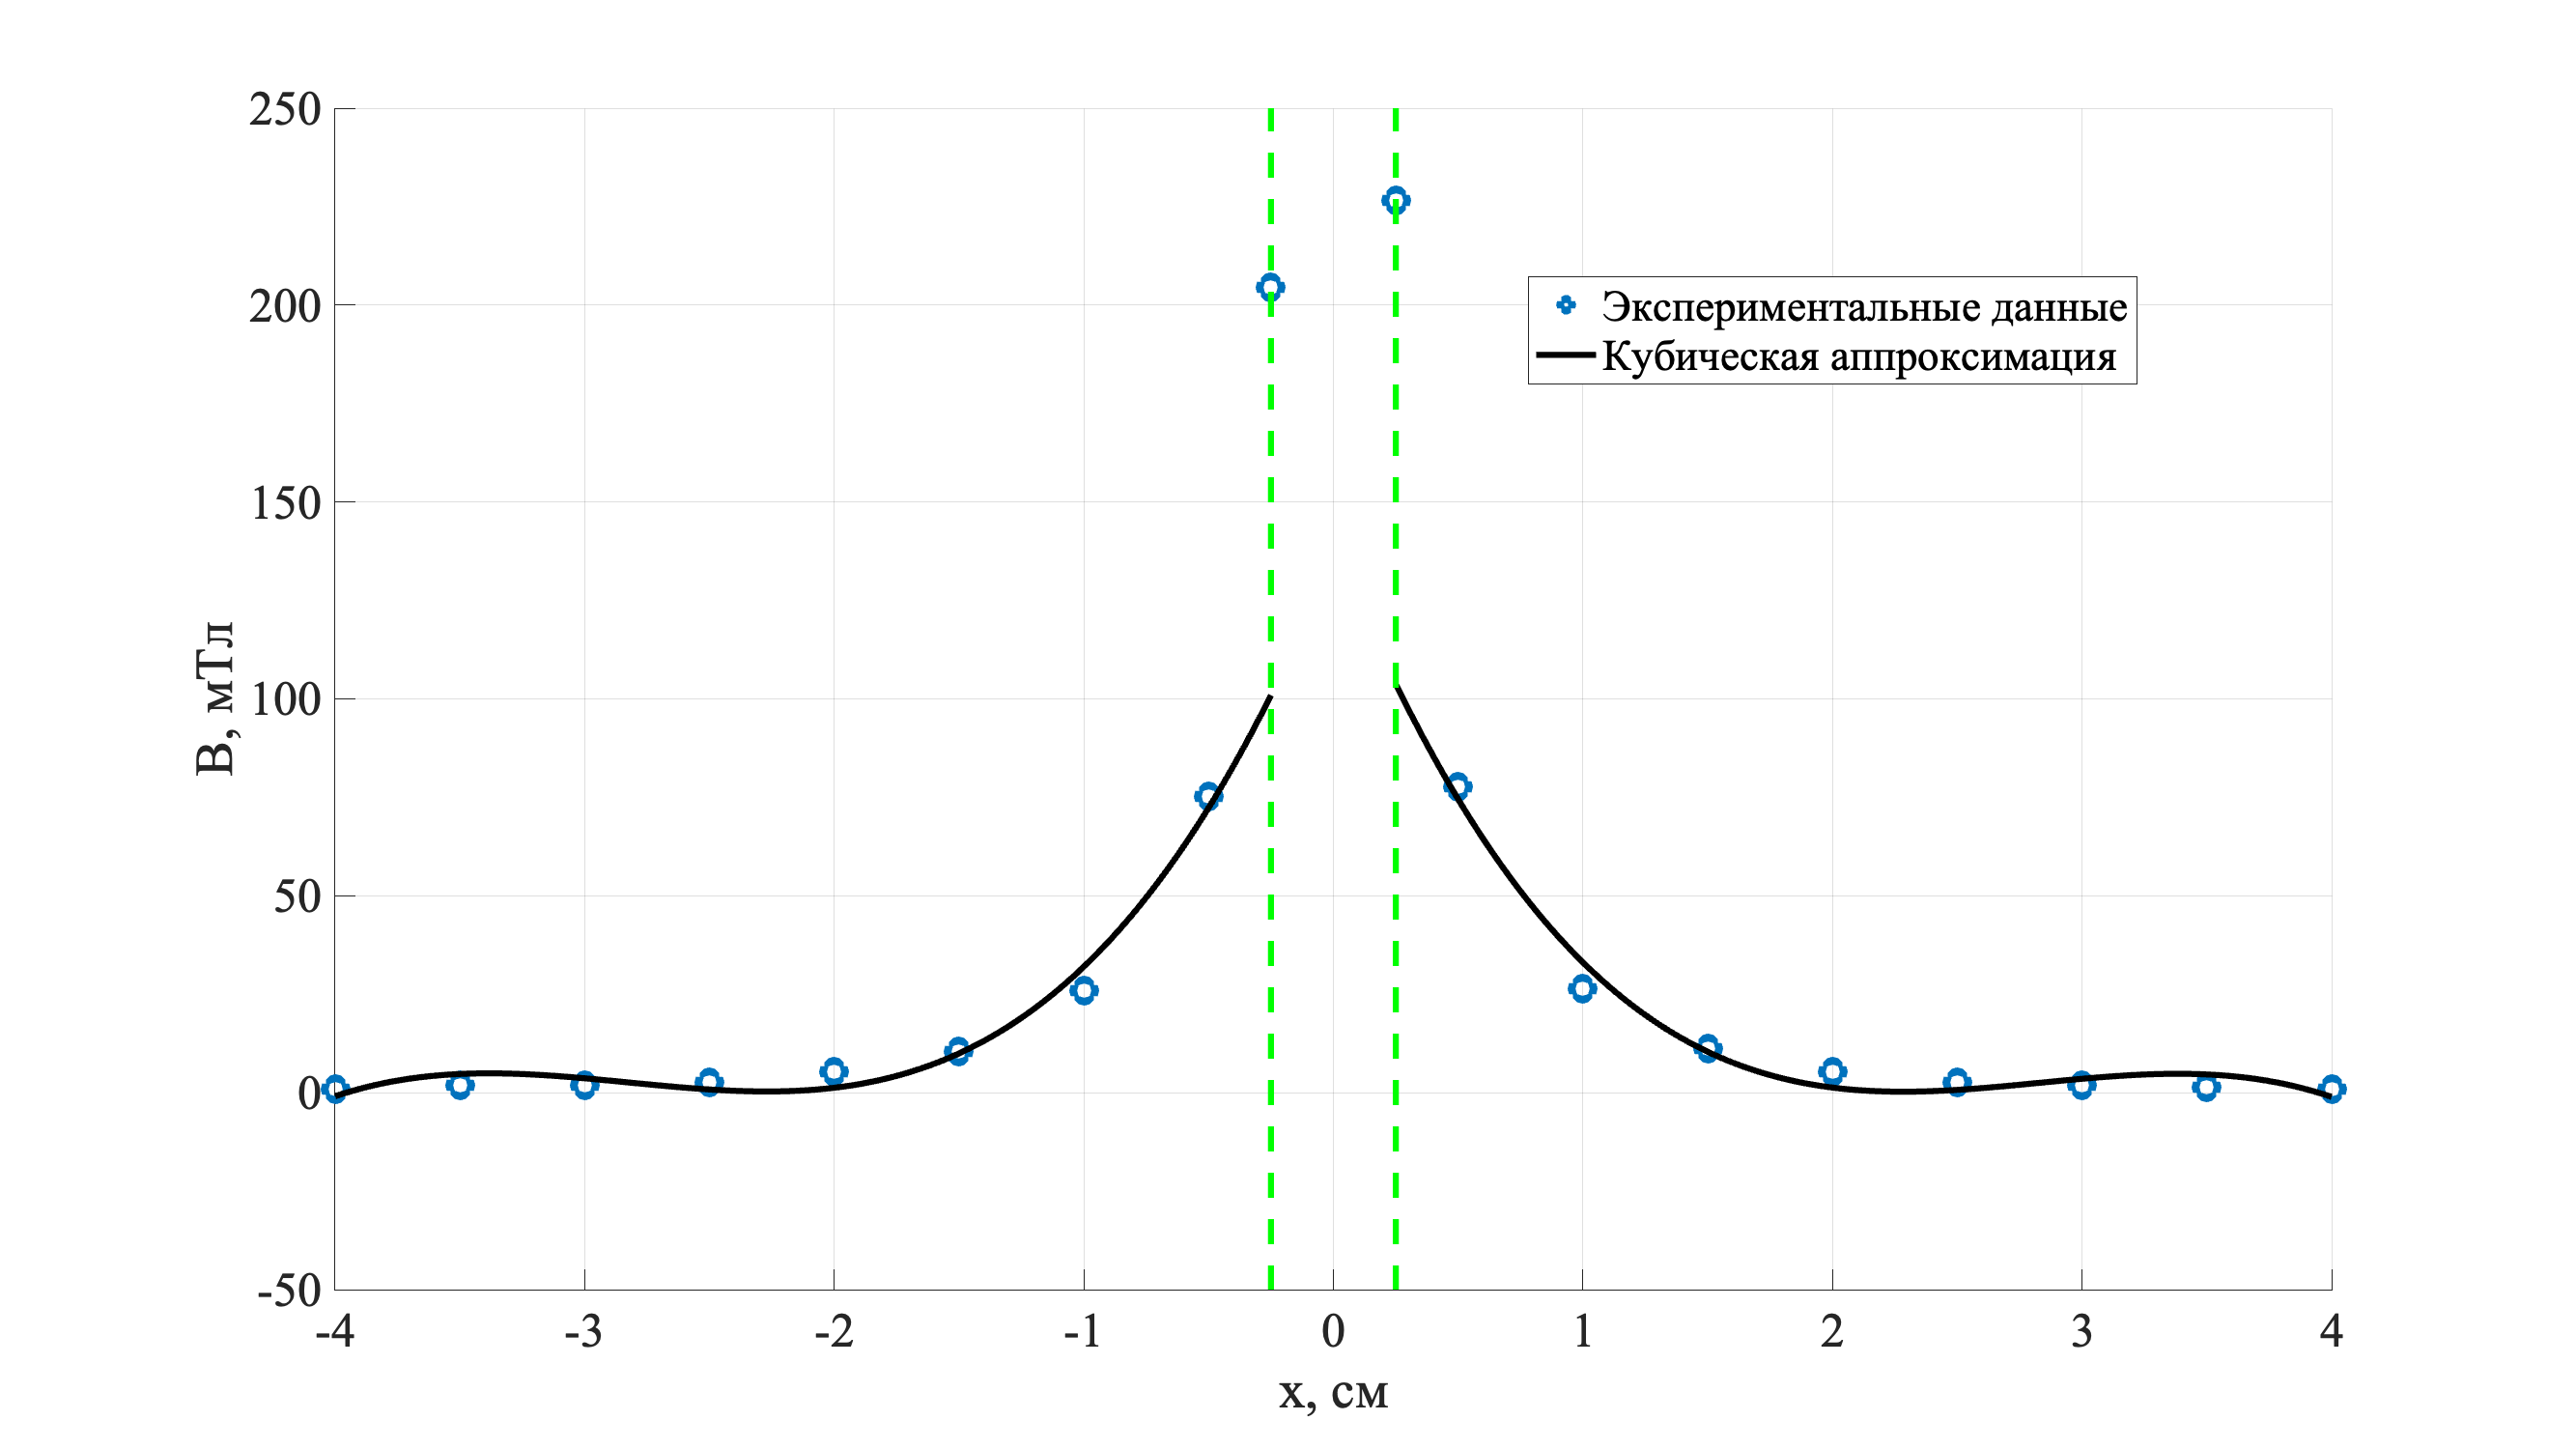
\includegraphics[width=1\textwidth]{plot3}
    \caption{Поле магнита}
    \label{fig:plot3}
\end{figure}

На примере соленоида убедимся, что справедлива формула:
\begin{equation}
	B = \frac{2\pi i}{c} (\cos\alpha_1 - \cos\alpha_2)
\end{equation}

Построим график зависимости поля от координаты:
\begin{figure}[h]
    \centering
    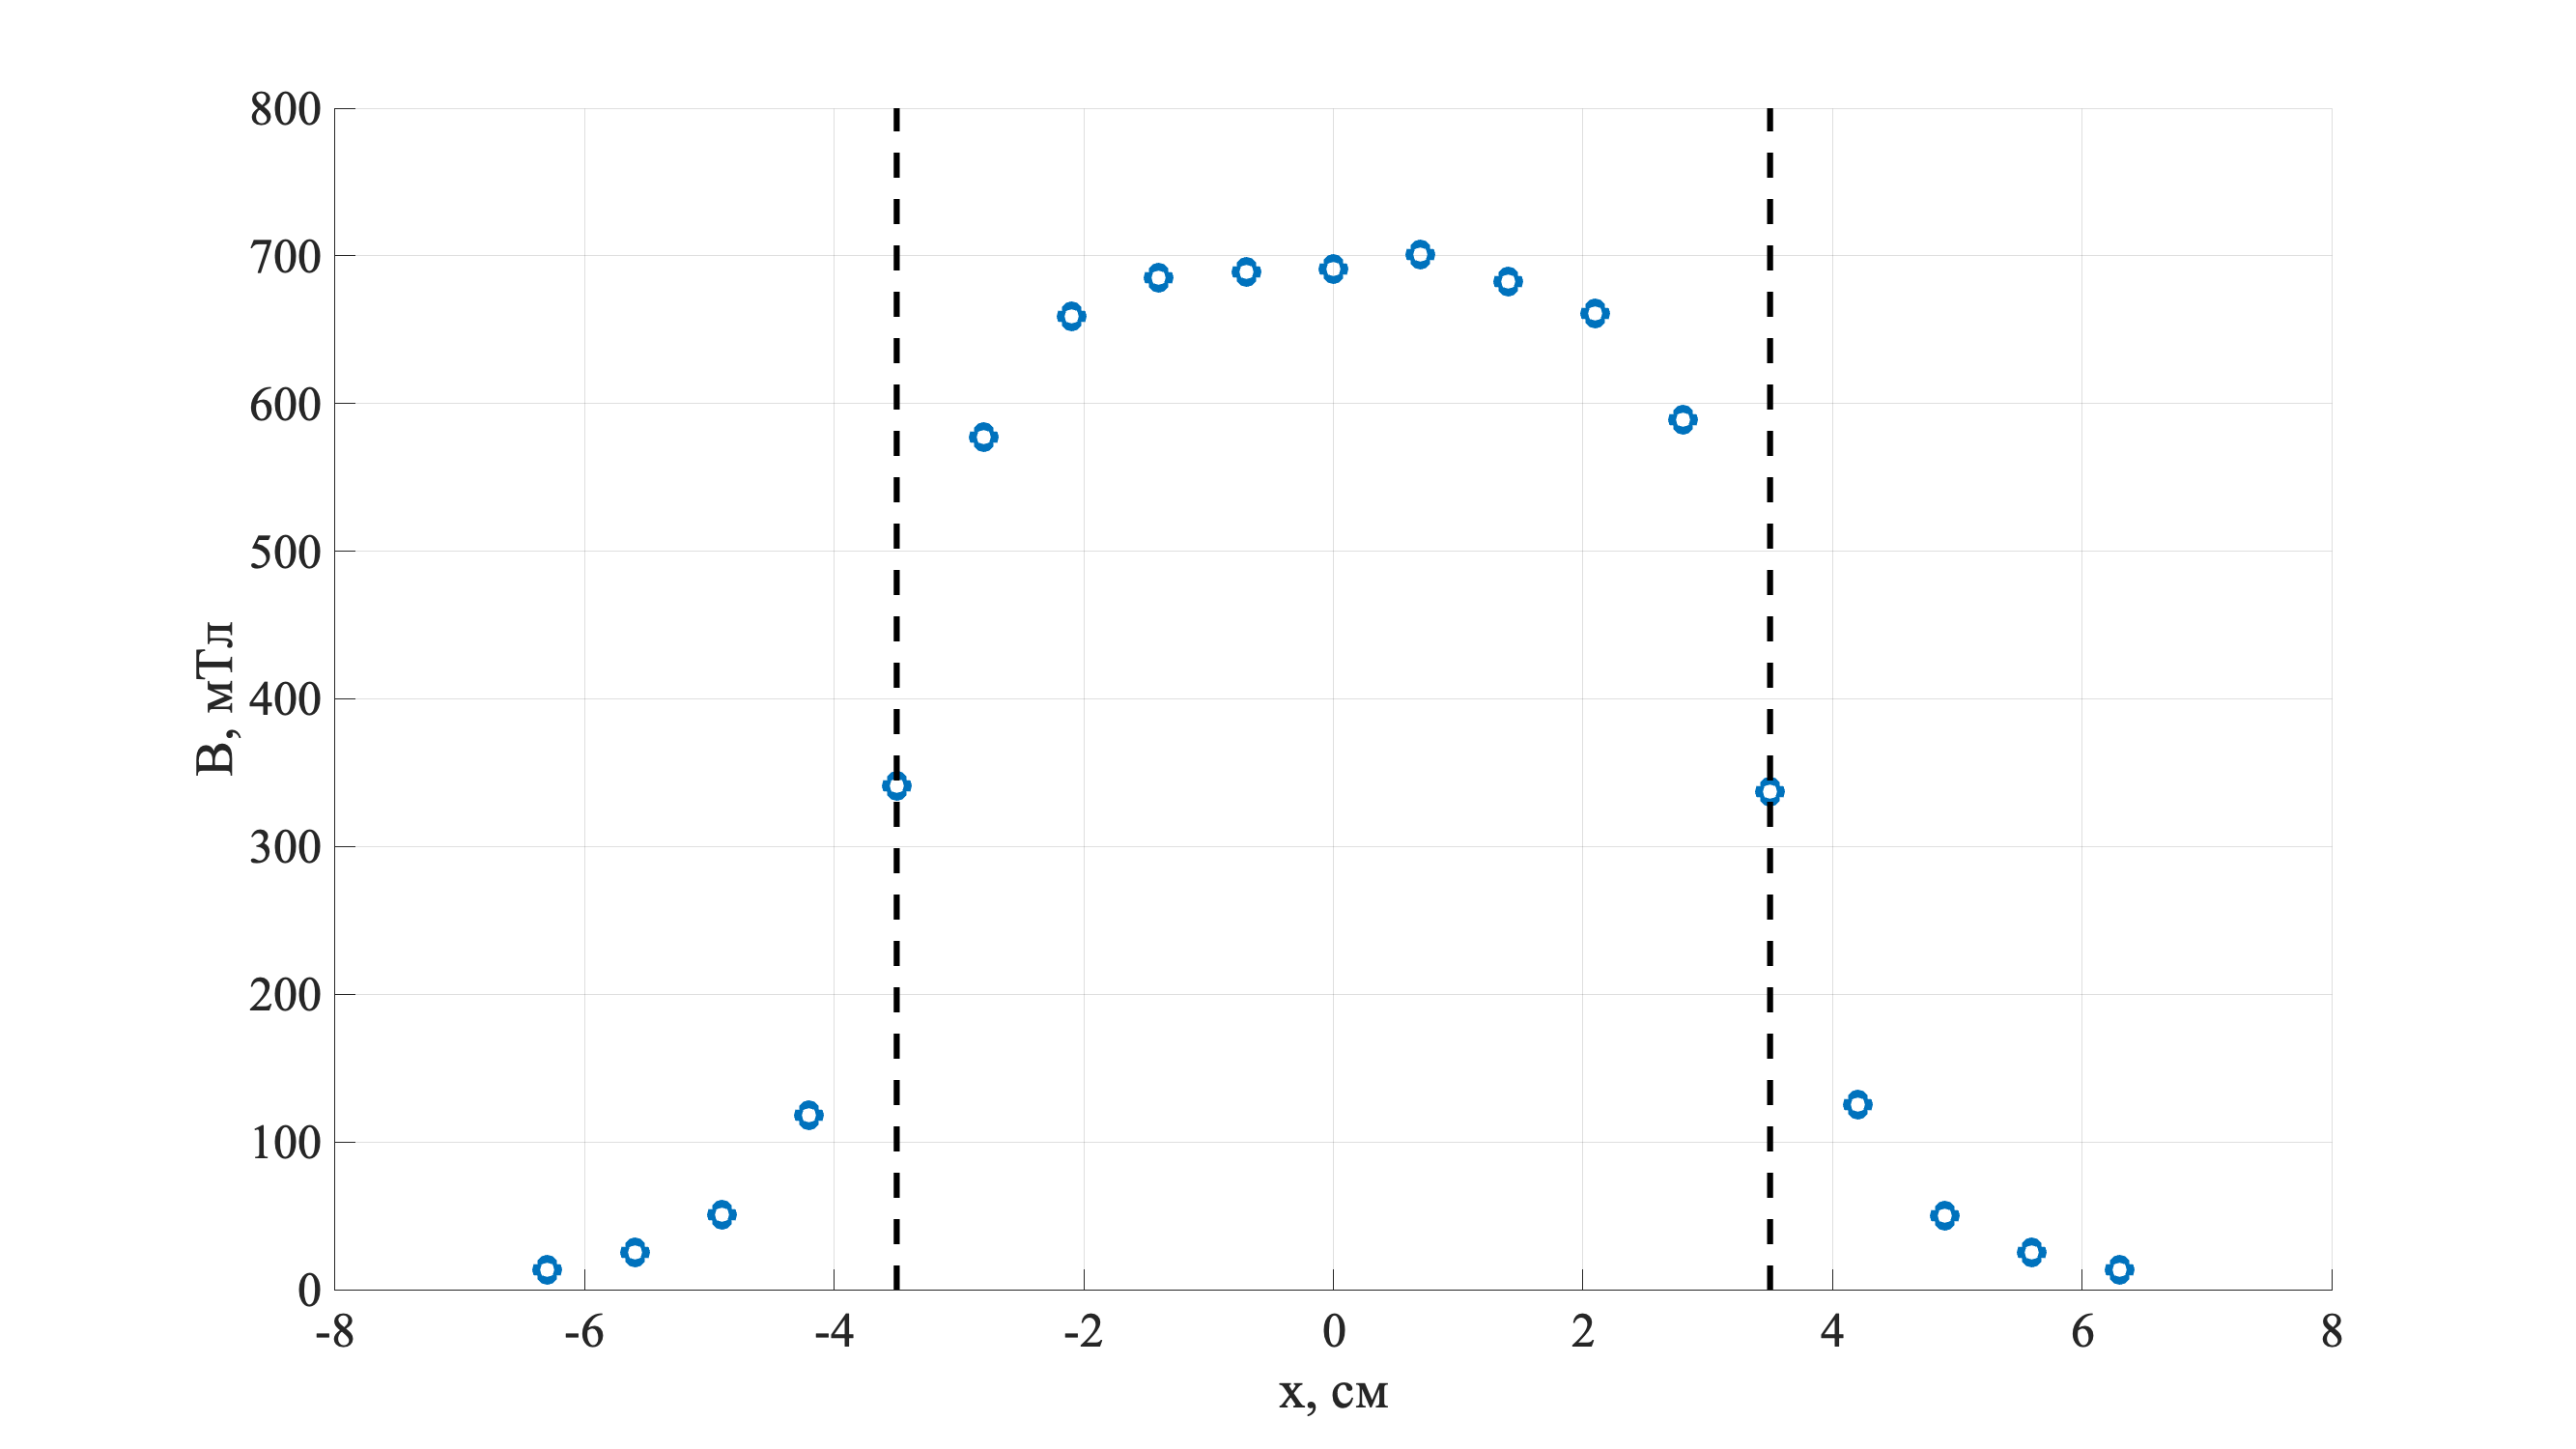
\includegraphics[width=1\textwidth]{plot4}
    \caption{Поле соленоида}
    \label{fig:plot4}
\end{figure}

\end{document}